\section{Review method}\label{sec:stoa:review-method}
In this section, the research method used to conduct this literature review is presented. We have used Covidence to manage the review process. Covidence is a web-based collaboration software platform that streamlines the production of systematic and other literature reviews~\cite{covidence}.

\subsection{Review question}\label{sec:stoa:review-questions}
The main research question for this systematic literature review is:

\begin{center}
    \textit{What is the state of the art in point cloud analysis, both classification and segmentation, of railway infrastructure?}
\end{center}	

\subsection{Data sources and search strategy} % Database selection
To select proper data sources to find articles for our literature review, the following database inclusion criteria were used:
\begin{itemize}
	\item that are pertinent to our research (only general databases, engineering databases or computer science specific databases)
	\item that have peer-reviewed articles
	\item that allow to search on phrases
\end{itemize}	

To extract paper relevant to the research question we have primarily used two databases:
\begin{itemize}
    \item Scopus \cite{scopus}
    \item Web of Science \cite{web-of-science}
\end{itemize}
We have also used three other databases to verify the completeness of information namely ACM~\cite{acm}, DBLP~\cite{dblp}, and IEEExplore~\cite{ieeexplore}.

The search query used for finding relevant literature was:
\begin{center}
    \textit{ (point cloud OR point clouds) AND railway}
\end{center}

We restricted the search to the papers' titles, abstracts, and keywords with a case-insensitive search. In Scopus, a total of 271 papers were found, and in Web of Science, 158 papers were found. Importing all these papers in Covidence resulted in 121 duplicates, thus leaving 308 papers for further review. We have manually checked the results from the other databases and compared them with the list generated in Covidence. This comparison did not reveal any new papers. 

\subsection{Study selection} 
The papers were further screened by reading the title and abstract. Only papers satisfying all criteria proceeded to a full-text review, the others were excluded. The following paper \textbf{inclusion} criteria were used:

\begin{enumerate}
    \item written in English or Dutch
    \item published in 2005 or later
    \item using outdoor data
    \item describing methods of analysing\slash pre-processing point clouds
    \item \label{stoa:inclusion-bridges} describing scenery reconstruction if the dataset contains tunnels/bridges
    \item describing transformation from point cloud to mesh
    \item describing Building Information Modelling of railway infrastructure
\end{enumerate}

Criterion~\ref{stoa:inclusion-bridges} was included after the observation during the abstract screening phase that some point cloud papers are only handling tunnels and bridges. The railway infrastructure was not specifically included. However, some examples contained parts of railways. This is observed mainly for papers focused on the deformation of railway tunnels, where the focus was on the tunnel structure instead of railway infrastructure such as railway lines or catenary arches.

The following paper \textbf{exclusion} criteria were used:

\begin{itemize}
    \item describing geometry in point clouds
    \item describing foreign object detection on the rail tracks
    \item short papers (less than four pages long)
\end{itemize}
	
Shorter papers, often less than four pages, may lack the comprehensive details and thoroughness found in longer articles, potentially offering only preliminary findings or lacking in-depth methodologies. Such papers might not have undergone the same rigorous peer review process as full-length articles, which is a vital step in ensuring the validity and quality of research. Therefore, to maintain the integrity and depth of our review, we have chosen to exclude papers less than four pages.\\

\paragraph{Screening process}
At the abstract and title screening stage, at least two assessors screened each paper. If the assessors disagreed on including or excluding the paper, a third assessor screened the title and abstract and decided the outcome. The procedure is applied to all 308 papers and resulted in the exclusion of 192 papers. Thus, 116 papers are left for the full-text review stage. 

A single assessor conducted the full-text review for each paper. Should there be any doubt regarding discarding a paper, it was referred to a second assessor. The rationale for a paper's rejection is duly recorded. Following this method, another 63 papers were excluded from the data extraction phase. This leaves 53 papers relevant to our research question which proceeded to the data extraction phase. Figure~\ref{fig:stoa:prisma} summarises the screening process and also detailing the number of papers excluded at each stage. 
\begin{figure}
    \centering
    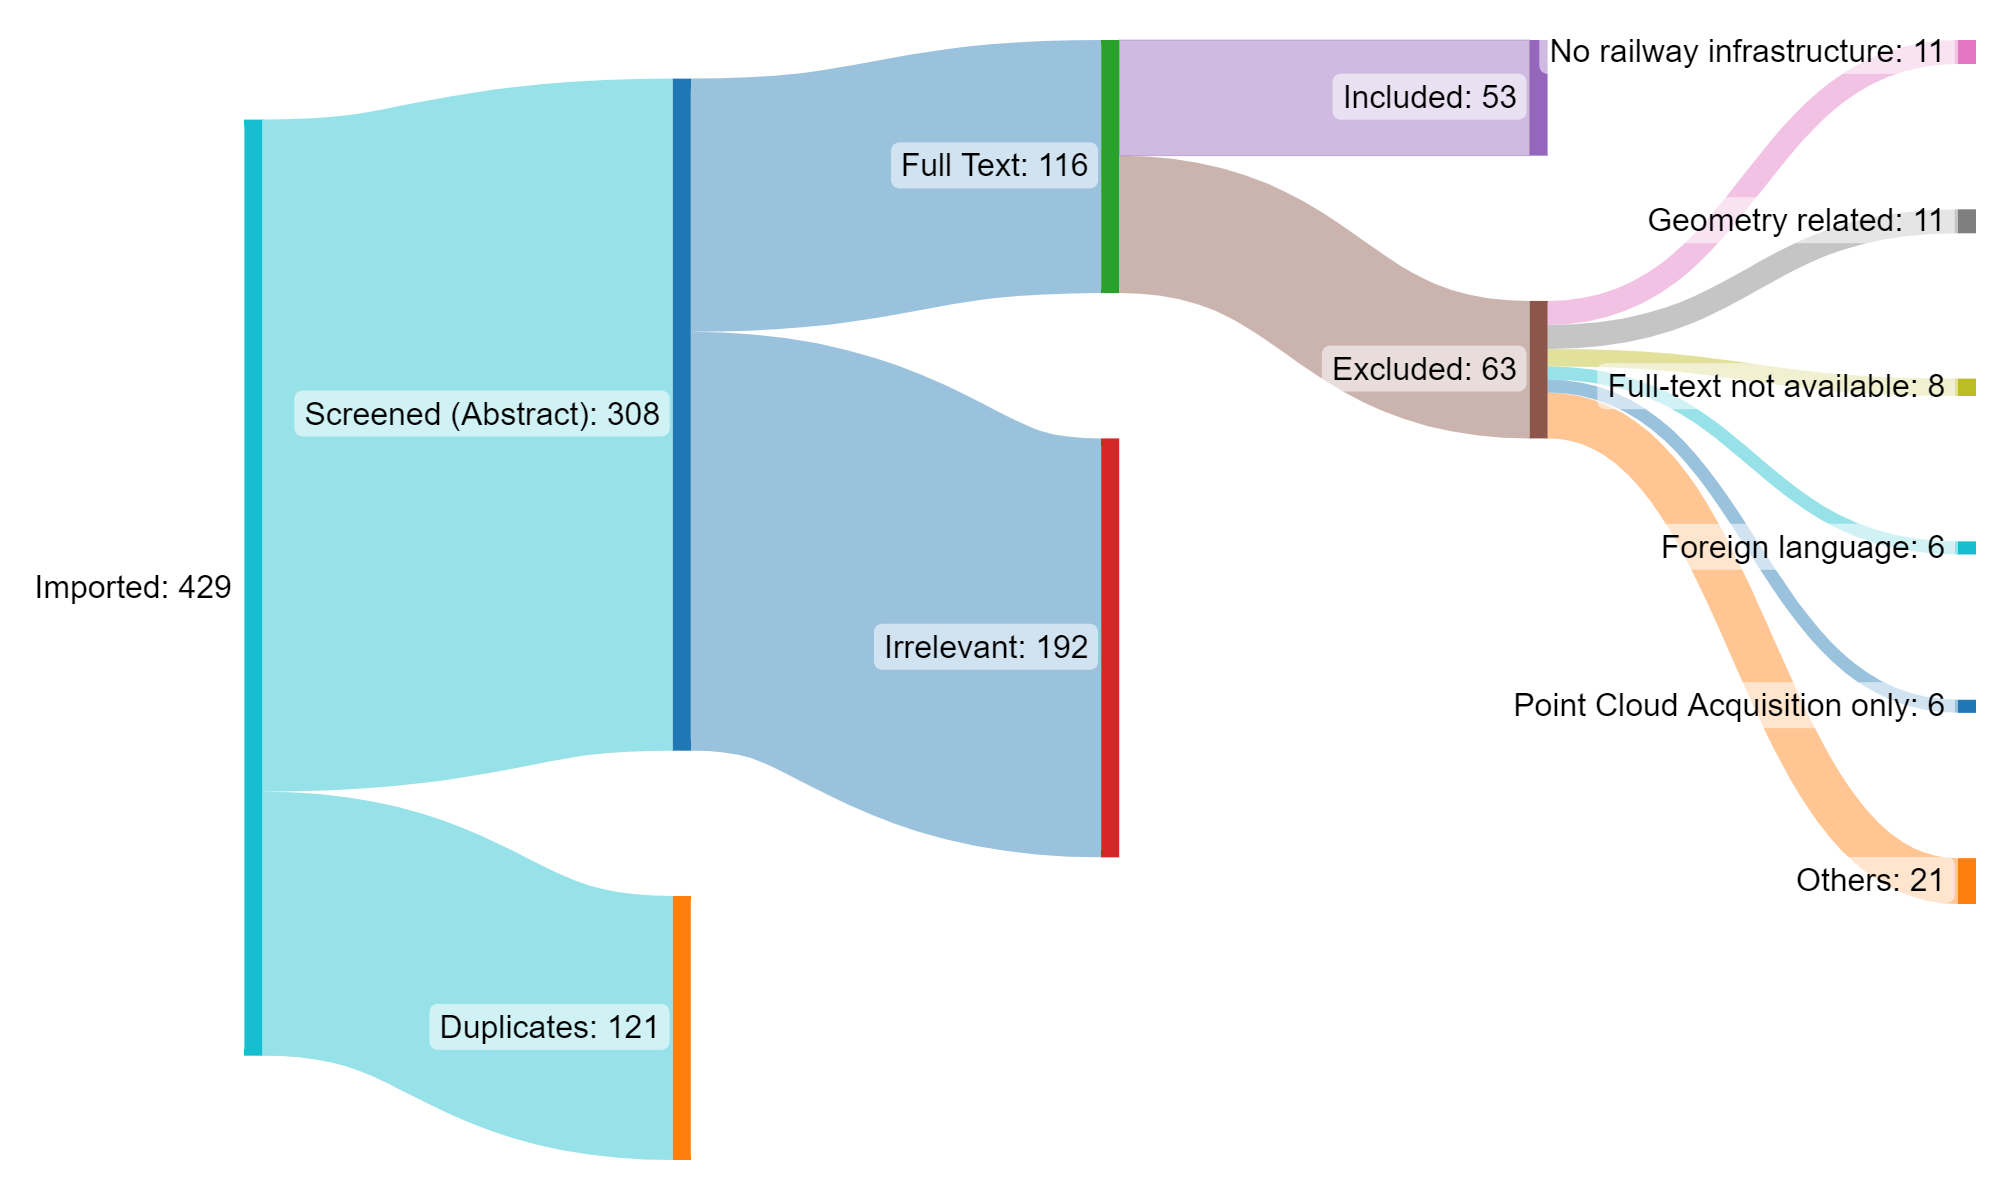
\includegraphics[width=0.95\linewidth]{./Chapters/stoa/fig/PrismaDiagram.png}
    \caption{An overview of the paper selection process with exclusion criteria.} 
    \label{fig:stoa:prisma}
\end{figure}

\subsection{Data extraction} % Extraction form used
In order to maintain the consistency of the data extraction process, we have used a form. The form is given in Table~\ref{tab:stoa:data-extraction}.
\begin{table}
    \centering
    \begin{tabular}{p{3.58cm}p{7.58cm}} %{|p{2.5cm}|p{8cm}|}
         \toprule
         \textbf{Field name} & \textbf{Description} \\
         \midrule
         Title & The title of the paper \\
         \addlinespace
         Goal & The main goal of the paper\\
         \addlinespace
         Steps & Which steps are described in the paper (pre-processing, modelling, digital twinning)? \\
         \addlinespace
         Pre-processing techniques & List the used pre-processing techniques \\
         \addlinespace
         Modelling techniques & List the used modelling techniques \\
         \addlinespace
         Digital twinning techniques & List the used digital twinning techniques \\
         \addlinespace
         Measurement of quality & What quality metrics are used? \\
         \addlinespace
         Country & From which country is the data in the dataset? \\
         \addlinespace
         Dataset & List characteristics of the dataset \\
         \addlinespace
         Experimental setup: speed & Speed of the vehicle while collecting the dataset\\
         \addlinespace
         Experimental setup: scanner type & Type of scanner used for collecting the dataset\\
         \addlinespace
         Experimental setup: RGB data & Are colours (or other additional information) present in the dataset?\\
         \addlinespace
         Notes & Any other relevant and interesting aspects\\
         \bottomrule
    \end{tabular}
    \caption{The data extraction form used for gathering useful information from every article.}
    \label{tab:stoa:data-extraction}
\end{table}
For the digitalisation of infrastructure, data collection plays a crucial role. Therefore, we have collected data reported in the selected studies related to data collection or meta-information. Most importantly, we collected the scan speed (speed of the vehicle if it is vehicle mounted), presence of colour information, or simultaneous collection of other sensory data such as GPS. Note that not all papers have described the data collection process. 

We divided infrastructure digitalisation into three stages. The first stage is pre-processing, where raw or filtered data is pre-processed for modelling purposes. The second stage is the modelling itself, while the last stage is the creation of digital twins. The `Steps' field is used to register which stages are described in the paper. The results section is also divided with respect to these stages.
The notes field is used to note down any other relevant information not covered by any other field. 